
\section{RESEARCH BACKGROUND AND JUSTIFYING THE TOPIC}
\subsection{Actuality of Research}
\subsubsection{Motivation}
The development and production of mobile robots is currently a rapidly growing field. Such robots are used both in the industrial sector and in everyday life. Research and development of mobile robots is being actively carried out to eliminate the consequences of natural and man-made disasters, for the needs of the military-industrial complex and space research. In this regard, the creation of mobile robots is not only a commercially profitable and scientifically significant direction, but also a strategically important task for the state and society as a whole.  

The history of their evolution reflects the achievements in the field of robotics. The list summarises the key milestones in the speed increase of mobile robots and the specifics of their applications. The increasing speed of mobile robots inevitably leads to increasing demands on their internal systems. This applies both to the power of actuators, the accuracy of sensor systems, and control algorithms\citep{turn0search0}.

\begin{itemize}
    \item \textbf{1966–1972: Shakey the Robot} - 0.3 m/s (1.1 km/h), one of the first autonomous robots with basic pathfinding.
    \item \textbf{1997: Nomad} - 0.4 m/s (1.44 km/h), designed for planetary exploration \citep{nomad1997}.
    \item \textbf{2012: RHex (Boston Dynamics)} - Reached speeds of 0.5 m/s (1.8 km/h) on rugged terrain with dynamic leg motion \citep{cheetah2012}.
    \item \textbf{2016: Boston Dynamics SpotMini} - 1.6 m/s (5.8 km/h), stable walking on uneven ground \citep{spot2016}.
    \item \textbf{2020: Boston Dynamics Cheetah 3} - 3 m/s (10.8 km/h), designed for rugged terrains and high-performance locomotion \citep{cheetah2012}.
    \item \textbf{2022: Unitree Go1} - Capable of running at 3.8 m/s (13.7 km/h), aimed at consumer and research markets \citep{unitreeGo1}.
    \item \textbf{2023: Ghost Robotics Vision 60} - Reached speeds of 3 m/s (10.8 km/h), built for military and industrial applications \citep{ghostVision60}.
\end{itemize}


Traditionally, robotic systems have relied on light sensors such as cameras and lidars to build a view of the environment. Unfortunately, cameras and lidars are not universally functional when faced with illuminated or structurally degraded cases. Despite consistent developments on photometric calibration\citep{PointLightYang}, camera distortion calibration \citep{Jin2019} 

\begin{figure}[H]
    \centering
    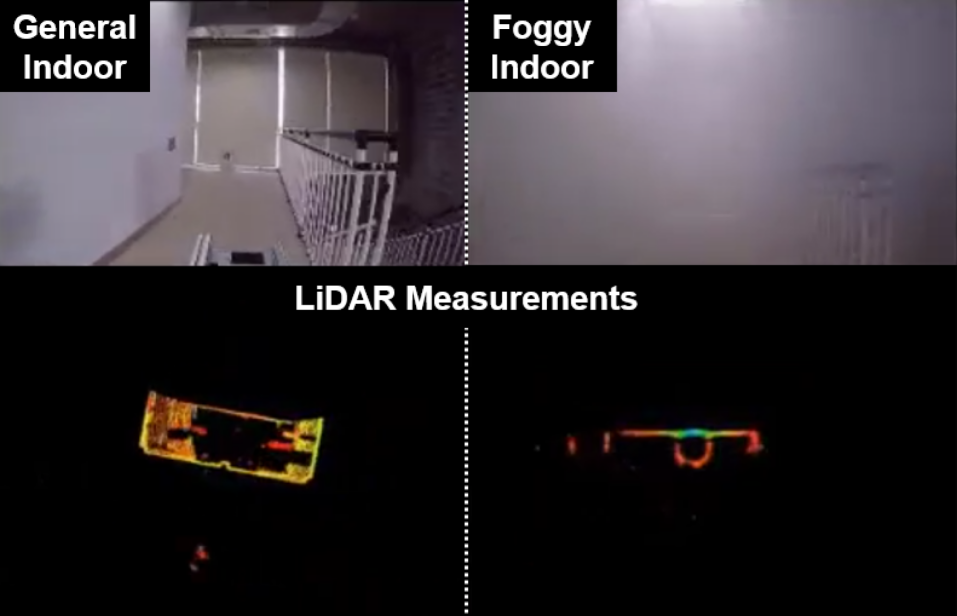
\includegraphics[width=\linewidth]{Src/images/x1.png} 
    \caption{Lidar measurements in a foggy indoor environment \citep{harlow2021mmwave}}
    \label{fig:lidarfogy}
\end{figure}
 
Navigational situations that seriously impair the camera \citep{starr2013navigation} and lidar \citep{radio1943detection} as seen on figure 1 but not the radar include smoke, dust, fog, rain, and snow. Radars can theoretically pass through the different types of tiny particulate matter by using longer wavelengths. 

Radar technology, although widely used in meteorology, target tracking, planetary mapping, and automotive safety, remains underutilized in robotics compared to shorter wavelength sensors like cameras and lidars. Radar systems transmit and receive specially shaped electromagnetic pulses to determine the distance and direction of objects, offering advanced sensing capabilities. This makes radar a valuable option for integration with existing systems or as an independent sensor, enabling robots to perform both metric and semantic tasks reliably.

The advent of mWave radars operating in the 76–81 GHz range provides a compact and alternative to lidar . 

\begin{figure}[H]
    \centering
    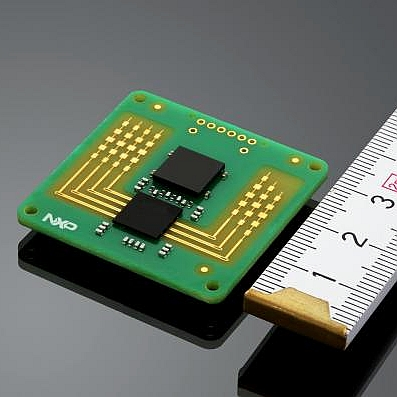
\includegraphics[width=\linewidth/2]{Src/images/automotive-radars.jpg} 
    \caption{Radar sensors \citep{tusur_radar_sensors}}
    \label{fig:radarsensor}
\end{figure}
In recent years, there has been a significant increase in the number of devices utilizing millimeter-wave (mmWave) radars. Most existing solutions are represented by radar-on-chip systems. A radar-on-chip is an integrated system that combines radar functionality into a single compact microchip device (Figure 1.2), making it applicable in various fields. Recent developments are focused on replacing presence sensors (PIR), with the primary goal being the detection of humans.\citep{s24113660}.

However, there are some reasons why robotics does not frequently use millimeter wave radars. Radar has numerous issues that need to be taken into account while creating new solutions, just like any other sensor. False reflections beyond the sensor's range, more intricate speckle noise, and multipath reflections—which produce several reflections from a single object—are just a few of the distinctive noise features of radar. 

Clustering-based filtering algorithms, such CFAR \citep{finn1968adaptive}, OPTICS \citep{nitzberg1972cfar}, and DBSCAN \citep{ankerst1999optics}, assist in reducing unwanted reflections and speckle noise, although require to be carefully tuned to fit particular hardware and antenna radiation patterns. Enhancing radar sensors themselves with greater resolution and quicker scanning rates can help with this to some extent. However, using various map formats, features, and internal state estimators also allows for algorithmic improvements.

The use of radar sensors in autonomous robots is an optimal solution because a robot is typically a complex collection of different systems. With other sensors, such as inertial sensors or odometers, the robot can determine its current speed, making it much easier to integrate and work with new types of sensors, including radar sensors. This allows for more reliable and accurate perception of the environment.

\subsubsection{Research Aim}
The aim of the work is to develop the principles of construction, as well as the algorithmic and software of the information radar system of a mobile robot.

 % Цель работы заключается в разработке принципов построения, а также алгоритмического и программного обеспечения информационной радарной системы мобильного робота.

\subsubsection{Objective of Research}
An information system for detecting and tracking fast-moving objects in robotics applications.
%Информационная система для обнаружения и отслеживания быстро движущихся объектов применительно к робототехнике.
\subsubsection{Subject of Research}
Mathematical models of navigation processes for the detection of selected dynamic objects using FMCW radar systems.
\section{State of the Art}
\subsection{Theoretical Understanding}
This section provides an overview of key mathematical tools that form the foundation of this thesis. It also establishes the notation and references for further exploration of the topic. The discussion begins with the concept of state estimation, focusing on two widely adopted state estimation methods in the field: the Kalman Filter and the Extended Kalman Filter. These techniques are introduced to highlight their significance and practical applications within the context of the research.
\subsubsection{Linear State estimation}

Dynamic systems are commonly represented in the time domain using state vectors, which encapsulate the internal state of a system at a given time \( t \). The state vector at the current time step, \( \mathbf{x}_t \), can be computed based on the previous state vector \( \mathbf{x}_{t-1} \), and optionally, a system input \( \mathbf{u}_t \). 
This relationship is expressed as:

\[
\mathbf{x}_t = \mathbf{A} \mathbf{x}_{t-1} + \mathbf{B} \mathbf{u}_t,
\]


where \( \mathbf{A} \), \( \mathbf{B} \), and \( \mathbf{C} \) are matrices that define the system dynamics, input influence, and output behavior, respectively. Additionally, the system output or measurement vector \( \mathbf{y}_t \) is derived from the current state as:

\[
\mathbf{x}_t = \mathbf{A} \mathbf{x}_{t-1} + \mathbf{B} \mathbf{u}_t,
\]

These matrices,\( \mathbf{A} \), \( \mathbf{B} \), and \( \mathbf{C} \) represent the linear behavior of the system, modeling its evolution, control input effects, and observable outputs, respectively \citep{welch2006kalman}.

In practical scenarios, it is rarely feasible to directly measure the true state variables of a system. This limitation arises due to noise, unobservable components, or inaccuracies in the model. To address this, uncertainties are typically represented using random variables, allowing probabilistic methods to quantify and manage such uncertainties. Continuous random variables, particularly in robotics, are often assumed to follow a normal (Gaussian) distribution. These distributions are characterized by their mean (expected value) \( \mu_t = \mathbf{x}_t \) and variance. When dealing with multiple state variables, covariance matrices \( \Sigma \) are used to represent the variances of individual variables as well as the covariances between them \citep{thrun2000probabilistic}.

The propagation of expected values follows deterministic rules defined by the system equations. Variance propagation, however, adheres to the error propagation laws \citep{siegwart2004robots}, incorporating additional noise \( \mathbf{R}_t \) from the system input. This results in the following relationship for covariance propagation:

\[
\Sigma_t = \mathbf{A} \Sigma_{t-1} \mathbf{A}^T + \mathbf{R}_t.
\]

The primary objective of state estimation techniques is to accurately approximate the state vector \( \mathbf{x}_t \) and provide reliable estimates of the associated uncertainties (variances) for each time step. These estimates are vital for analyzing and controlling dynamic systems effectively.

\subsubsection{Linear Kalman Filter} 


The Kalman filter is a widely used tool for processing noisy measurement data and predicting the state of a system based on input observations. Specifically, it is designed for continuous systems and, as noted in \citep{thrun2000probabilistic}, “is not applicable to discrete or hybrid state spaces.” The filter is particularly advantageous in real-time applications due to its recursive structure and computational efficiency \citep{welch2006kalman}. The Kalman filter consists of two primary steps: the prediction step and the update step. 

The \textit{prediction step} advances the current state estimate and covariance matrix to the next time step, using the equations of the system's dynamic model. 
The \textit{update step}, on the other hand, refines these estimates by incorporating the actual measurements and comparing them with the predicted output. The discrepancy between the predicted and observed outputs is adjusted using the Kalman Gain \( \mathbf{K}_t \), which is derived from the covariance of the prior state \( \Sigma_{t-1} \), process noise \( \mathbf{R}_t \), and measurement noise \( \mathbf{Q}_t \).

The linear Kalman filter assumes linear system dynamics, unimodal Gaussian state distributions, and uncorrelated, zero-mean noise \citep{welch2006kalman}. Starting from the initial state \( \mathbf{x}_0 \) and covariance matrix \( \Sigma_0 \), the filter recursively updates the current state \( \mathbf{x}_t \) and covariance \( \Sigma_t \) based on the input data \( \mathbf{u}_t \), measurement \( \mathbf{y}_t \), and noise covariances \( \mathbf{R}_t \) and \( \mathbf{Q}_t \). The recursive algorithm is detailed in Algorithm~\ref{alg:kalman_filter}.


The filter's behavior is significantly influenced by the selection of process noise \( \mathbf{R}_t \) and measurement noise \( \mathbf{Q}_t \). Lower measurement noise covariance values \( \mathbf{Q}_t \) lead to greater reliance on measurements, resulting in faster adaptation to changes in system output. Conversely, smaller process noise \( \mathbf{R}_t \) indicates higher trust in the system model, promoting smoother results \citep{balzer2018kalman}. Both covariances can be determined either statically or dynamically. The static approach typically involves pre-measuring the measurement noise covariance, while process noise is more challenging to estimate and often requires fine-tuning \citep{welch2006kalman}. Advanced methods can dynamically adjust these covariances using adaptive techniques, such as leveraging prior filter estimates \citep{welch2006kalman}.


\subsubsection{Non-Linear State estimation}

Real-world systems include non-linear terms that cannot be transformed into a linear form. These systems are generally represented by the following equations:
\[
\mathbf{x}_t = g(\mathbf{u}_t, \mathbf{x}_{t-1}), \tag{2.9}
\]
\[
\mathbf{y}_t = h(\mathbf{x}_t). \tag{2.10}
\]

Here, the non-linear functions \( g \) and \( h \) replace the linear matrices \( \mathbf{A} \), \( \mathbf{B} \), and \( \mathbf{C} \), modeling the system dynamics and output behavior, respectively. To handle these non-linearities, the functions \( g \) and \( h \) can be approximated at each time step using a first-order Taylor expansion. This results in the computation of the Jacobian matrices \( \mathbf{G}_t \) and \( \mathbf{H}_t \), which correspond to a linear tangent at the non-linear functions, calculated as the partial derivatives (gradients) at the current state value \citep{thrun2000probabilistic}:

\[
\mathbf{G}_t = \frac{\partial g(\mathbf{u}_t, \mathbf{x}_{t-1})}{\partial \mathbf{x}_{t-1}}, \tag{2.11}
\]
\[
\mathbf{H}_t = \frac{\partial h(\mathbf{x}_t)}{\partial \mathbf{x}_t}. \tag{2.12}
\]

As with linear systems, the process is subject to perturbations from system noise and measurement noise, represented by the random variables \( \mathbf{w}_t \) and \( \mathbf{v}_t \), respectively. The random influences of \( \mathbf{w}_t \) and \( \mathbf{v}_t \) can also be approximated using Jacobian matrices \citep{welch2006kalman}:

\[
\mathbf{W}_t = \frac{\partial g(\mathbf{u}_t, \mathbf{x}_{t-1})}{\partial \mathbf{w}_t}, \tag{2.13}
\]
\[
\mathbf{V}_t = \frac{\partial h(\mathbf{x}_t)}{\partial \mathbf{v}_t}. \tag{2.14}
\]

Unfortunately, most non-linear functions disrupt the Gaussian property of the state distribution. To preserve this critical characteristic, an approximation of the system function \( g \) is used by employing the Jacobian matrices \( \mathbf{G}_t \) and \( \mathbf{W}_t \) for error propagation \citep{welch2006kalman}:

\[
\Sigma_t = \mathbf{G}_t \Sigma_{t-1} \mathbf{G}_t^T + \mathbf{W}_t \mathbf{R}_t \mathbf{W}_t^T. \tag{2.15}
\]

This approach enables the handling of non-linear systems while maintaining the Gaussian assumption, which is essential for the performance and stability of state estimation methods.

\subsubsection{Extended Kalman Filter}


The Extended Kalman Filter (EKF) generalizes the concept of the linear Kalman Filter to handle non-linear systems. It utilizes the approach presented in Eq.~(2.15), where error propagation is approximated using Jacobian matrices to preserve the Gaussian property of the state distribution. The EKF algorithm (Algorithm~\ref{alg:ekf}) closely resembles its linear counterpart (Algorithm~\ref{alg:kalman_filter}).



The selection of process noise covariance \( \mathbf{R}_t \) and measurement noise covariance \( \mathbf{Q}_t \) in the EKF is analogous to the linear Kalman Filter. Like its linear counterpart, the EKF assumes a Gaussian distribution with zero-mean, uncorrelated noise. Despite these assumptions, it has been successfully applied to numerous state estimation problems that violate these underlying conditions \citep{thrun2000probabilistic}.

While the EKF is a widely used state estimator in robotics, it is important to acknowledge its limitations. The accuracy of the filter depends heavily on the quality of the linearization, which may become poor for systems with highly non-linear or multi-modal functions \citep{thrun2000probabilistic}. This can lead to suboptimal performance in such scenarios, highlighting the importance of understanding the system dynamics before relying on the EKF.

\subsection{Object Motion}

\subsubsection{Range sensors}
\subsubsection*{LiDAR}

\cite{Mertz2013} provide a good, though somewhat outdated, overview of different approaches to DETECT AND TRACK MOVING OBJECTS (DATMO) using laser scanners. They distinguish between 2D, 2D+ (laser scanners with four scanning planes) and 3D systems.

% The most obvious way to identify objects is to utilize distance sensors. Different physical principles underlie the many types of sensors. The most often used systems in robotics are LiDAR, ultrasonic, and infrared system. While LiDAR systems continue to be a popular option for DETECT AND TRACK MOVING OBJECTS (DATMO) operations, the first two sensor types are less effective than LiDAR in terms of operating circumstances and resolution.
% \begin{figure}[H]
%     \centering
%     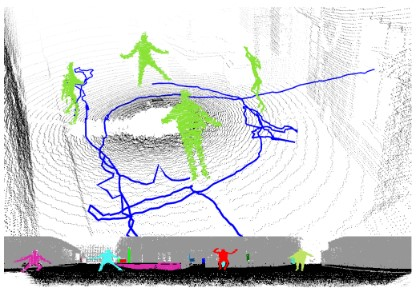
\includegraphics[width=\linewidth/2]{img/Screenshot 2025-01-07 142952.jpg} 
%     \caption{Lidar data segmentation\citep{Lichtenfeld2024}}
%     \label{fig:radarsensor}
% \end{figure}
% Point grouping, segmentation, data matching, and track updating are the four general processes of LiDAR DATMO techniques \citep{Lichtenfeld2024}. To find a cluster, the data from each survey is first clustered based on predetermined metrics, such as Euclidean distance or intensity. The freshly created clusters are then compared to the tracks of previously tracked items during time.


\subsubsection{Camera sensors}
\paragraph{Monocular Camera}
Vision systems are divided into those using one (monoculars) and more than one video camera. The operation of vision systems using several video cameras is based on the comparison of images of the external environment obtained from two or more spatially separated points of the mobile robot. Due to the spatial separation of the received images in such vision systems, the necessary information about the spatial characteristics of the object is determined. 
% \begin{figure}[H]
%     \centering
%     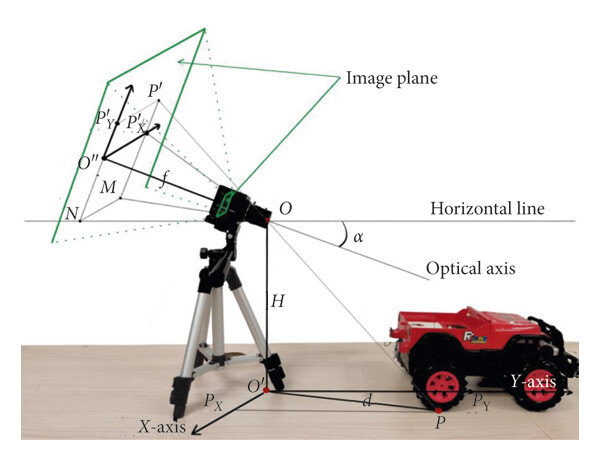
\includegraphics[width=\linewidth/2]{img/scpr9979111-fig-0003-m.jpg} 
%     \caption{Monocular Vision Ranging\citep{xue2021monocular}}
%     \label{fig:radarsensor}
% \end{figure}
A separate video camera for determining distances to stationary objects can be integrated into the navigation system of a mobile robot. Such a camera focuses on collecting visual data, which is then analyzed to calculate distances to static objects in the robot's environment.

The use of an additional device can reduce the load on the main image processing system, improve the accuracy of measurements, and improve the reliability of the robot. The specialized camera can be optimized in terms of weight and dimensions, which is especially important in the design of mobile devices where compactness and low weight are critical. At the same time, the robustness and stability of the camera design ensure correct operation in various environments, ensuring stable dimensioning and distance to fixed objects.

\paragraph{Stereo Camera}
It is possible to calculate a difference map and extract 3D information from the stereo camera system given two images with a defined baseline. This 3D data makes it possible to specify motion characteristics and measure an object's physical attributes directly.
% \begin{figure}[H]
%     \centering
%     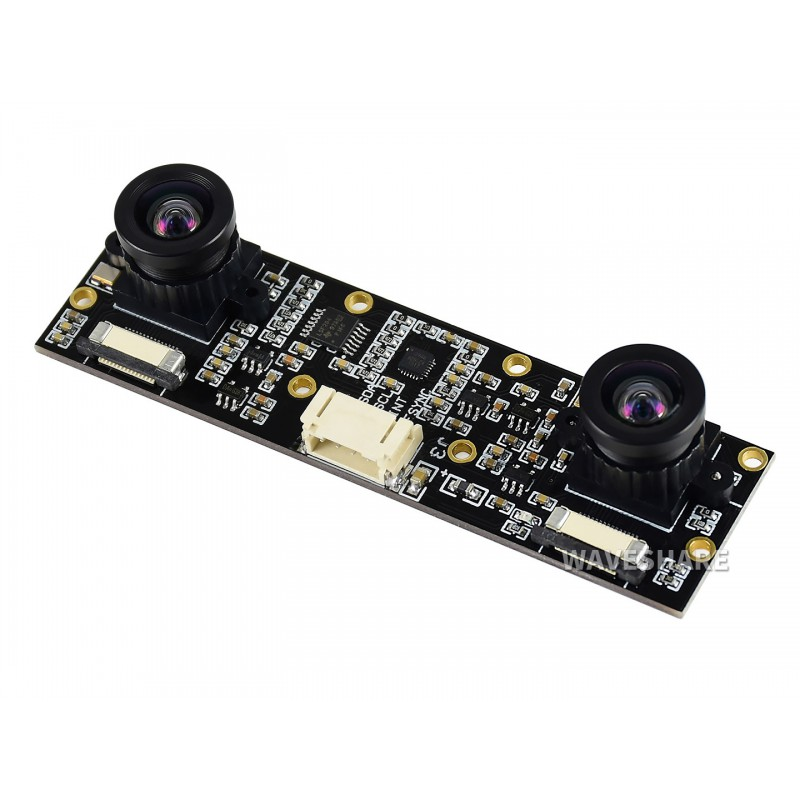
\includegraphics[width=\linewidth/2]{img/imx219-83-stereo-camera-1.jpg} 
%     \caption{Stereo Camera Module}
%     \label{fig:radarsensor}
% \end{figure}

\subsection{Ego-Motion}
This is the process of determining the self-motion of a camera or robot in space relative to its environment. Technologies that use sequential image analysis and sensor data to calculate changes in the position and orientation of an object.
\subsubsection{Inertial systems}
Similar to the dead reckoning method, inertial navigation systems (INS) obtain pose information by integrating sensor data \citep{biezad1999integrated}. But instead of integrating velocity, ANNs utilize the properties of inertia. Inertial sensors such as INSU (Inertial Measurement Units) give acceleration and angular velocity readings. In order to extract pose data, the acceleration must be indexed twice and the angular velocity must be indexed once \citep{grewal2020global}. 

% \begin{figure}[H]
%     \centering
%     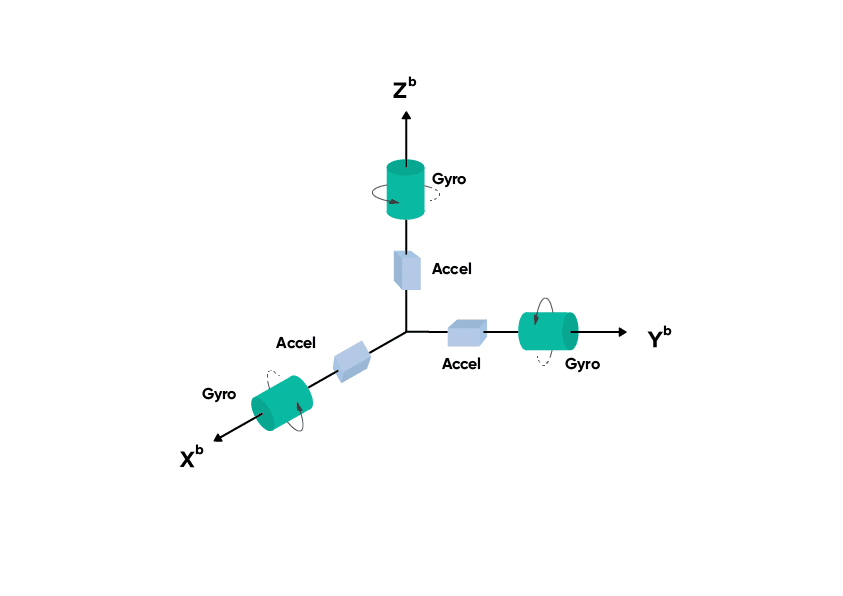
\includegraphics[width=\linewidth]{img/inertial-navigation-systems-ins-an-introduction-img001.png}
%     \caption{INS}
%     \label{fig:INS}
% \end{figure}

Thus, an ANN is a combination of a sensor and a computing device that performs data filtering and integration. Compared to odometry or dead reckoning, ANN is a relatively new trend in robotics that has emerged due to the recent emergence of accurate and affordable sensors \citep{Borenstein1996WhereAI}.

\paragraph{Inertial Measurement Unit} are widely used in robotics to measure angular velocities using gyroscopes and accelerations along three axes. Such devices, made by MEMS technology, are cheap, compact, reliable and low-consumption \citep{biezad1999integrated}. IMUs are usually attached rigidly to the robot, so they are called strapdown systems. They detect changes in velocity and orientation relative to the global coordinate system\citep{biezad1999integrated}.

To track the current pose, the system first integrates angular velocities to determine orientation. The measured accelerations are then converted to the global coordinate system with the influence of gravity removed. This approach allows to accurately determine the position and orientation of the robot in space.


\subsubsection{Odometry}
Dead reckoning and odometry are two concepts that are not always easily distinguished. The process of estimating the present pose by integrating velocity and a known heading is sometimes referred to as dead reckoning. Conversely, odometry usually means figuring out the present position using information from "odometer" sensor, the total number of traveled path segments that is acquired from an encoder \citep{Borenstein1996WhereAI}. These phrases are commonly used interchangeably, albeit their definitions can differ. In this thesis, dead reckoning refers to determining the pose by integrating velocity data, whereas odometry particularly refers to calculating the robot's pose by adding up incremental path segments. Both approaches are simple and popular ways to find the position and orientation of a robot \citep{Scaramuzza2011}.

\paragraph{Encoder Sensors}
In robotics and control systems, encoders are frequently employed to precisely determine the location and velocity of spinning components. By converting mechanical motion into digital information, encoders make it possible to measure changes in shaft speed, angle, or distance traveled. Measurements are provided by optical or magnetic encoders in modern devices  \citep{Smith2019} .They are capable of measuring absolute or relative. Using the vehicle's geometric characteristics, such as wheel diameter and gear ratio, the recorded angle can be translated into the robot's trip distance \citep{Doe2020}.
They are extremely challenging to detect quantitatively and to test for \citep{Borenstein1994UMBmarkA}. On the other hand, systematic errors are simpler to handle. They result from inaccurate mechanical components, inadequate comprehension of the system, or approximations in system models. Various calibration methods can be used to estimate and reduce them.

\paragraph{Optical Speed Sensors}
Another motion detection technique uses optical sensors and image processing to measure movement speed directly on a 2D surface. This kind of sensor is usually sold as an off-the-shelf device with integrated image processing algorithms, making it simple to access the motion data in its raw form. This technique has the advantage of non-contact measuring, which eliminates the need for mechanical errors and backlashes. This concept of functioning is used by two major kinds of sensors.

On the one hand, cheap optical motion sensors are frequently found in computer mouse. They are small, use only a few milliwatts of electricity, and have a 10 m/s speed detection range \citep{Logitech2020}. The requirement for a "cooperative" surface, calibration for every individual surface, and a relatively small fixed measured distance are some of the major drawbacks of such sensors.
% \begin{figure}[H]
%     \centering
%     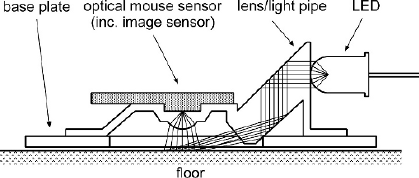
\includegraphics[width=\linewidth/2]{img/Structure-of-optical-mouse-sensor.png}
%     \caption{Structure of optical mouse sensor}
%     \label{fig:optical}
% \end{figure}
And High-performance solutions, on the other hand, are employed as reference systems in vehicle dynamics research \citep{SensoricSolutions}. Despite their great precision in dry conditions on a level surface, these sensors are relatively big and costly.


\subsubsection{Visual Odometry}
Visual odometry is a method of estimating the motion of a robot using sequential images from cameras or lidars \citep{Scaramuzza2011}.

\paragraph{Waypoint Navigation Systems}
Navigation systems based on waypoint traversal are currently among the most reliable. However, they have several obvious limitations that significantly restrict their applications. Primarily, these systems are confined to limited spaces, usually indoors, and are prone to errors when unforeseen obstacles appear within the robot's operating area \citep{Borenstein1996WhereAI}. Additionally, maintaining the waypoints (or beacons) requires regular servicing.

% \begin{figure}[H]
%     \centering
%     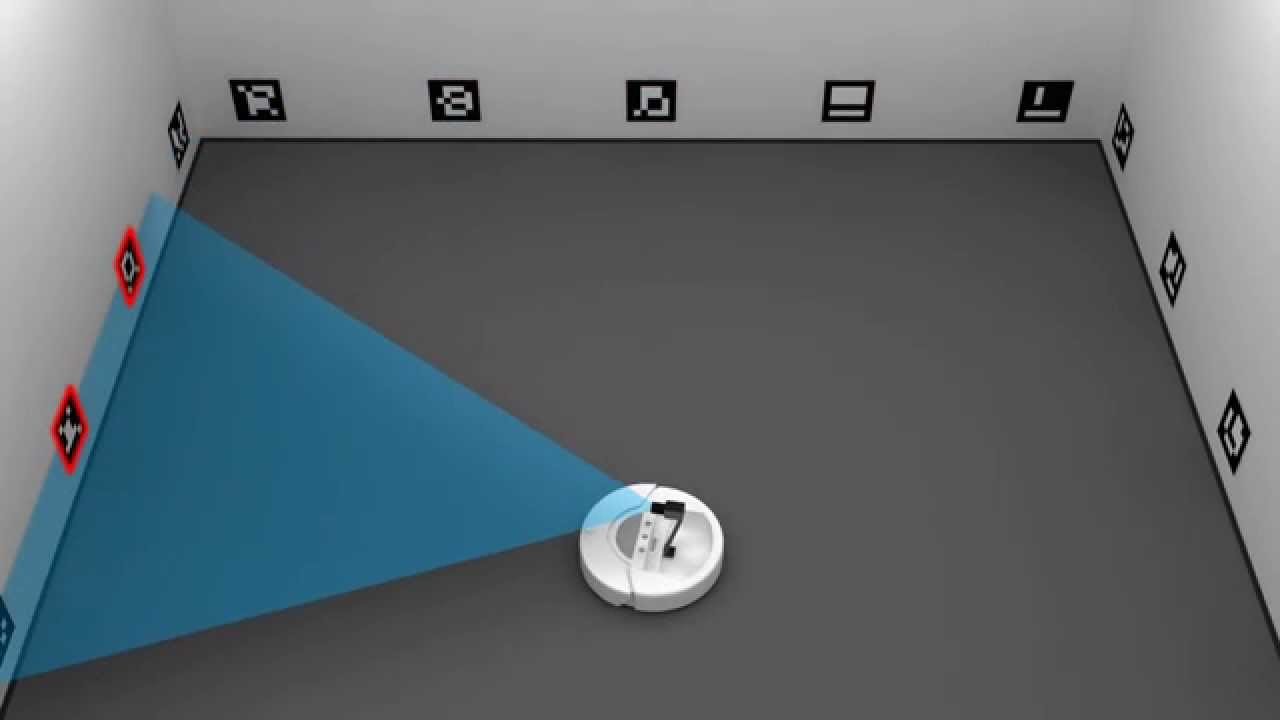
\includegraphics[width=\linewidth/2]{img/maxresdefault.jpg}
%     \caption{Robot Localization using Waypoint Navigation Systems}
%     \label{fig:Waypoint}
% \end{figure}

\paragraph{Laser and Ultrasonic Range Sensors}
Another class of rangefinders commonly used in small-scale robots includes laser and ultrasonic range sensors. These are typically employed indoors to perform simple tasks within structured environments . Lidars are limited by the fact that the laser beam only captures data within its line of sight. Small interferences along the beam path can introduce inaccuracies into the generated environmental representation. Ultrasonic sensors, on the other hand, suffer from relatively slow response times, particularly in large open spaces. This limitation prevents robots from moving quickly in such environments.

\subsubsection{Light Sensor-Based Systems}
Light sensors range from basic photo-sensitive elements to more sophisticated systems employing video cameras.

\paragraph{Photo-Sensitive Elements}
Photo-sensitive elements include components such as photoresistors or infrared (IR) and ultraviolet (UV) receivers. The principle of photoresistors relies on the reduction of resistance with increasing illumination. IR and UV sensors detect obstacles by analyzing light reflected from objects. Using IR and UV LEDs and sensors, obstacles can be detected even before contact because ambient light typically contains minimal radiation at these wavelengths \citep{Logitech2020, SensoricSolutions}.

\paragraph{Vision-Based Systems}
Navigation systems that employ video cameras to extract spatial information about the surrounding environment, known as vision-based systems, are particularly noteworthy. Developing such systems is a challenging task, often situated at the intersection of multiple disciplines within artificial intelligence \citep{Jin2019, PointLightYang}. These systems are highly versatile and, in theory, can be equally effective in both indoor and outdoor environments. However, their reliability remains insufficient due to several factors, including susceptibility to various interferences (e.g., vibrations, atmospheric disturbances, optical distortions), the high volume of data to be processed, and the complexity of analyzing the information. These challenges are primarily associated with object recognition issues in the camera's captured images.

The information processing in such systems generally mimics the human visual apparatus. Spatial data, including obstacle dimensions and distances, is obtained by comparing images captured from two or more viewpoints (stereo vision systems). Based on the disparities between these images, the necessary spatial characteristics of objects are calculated \citep{Smith2019, Doe2020}.

\paragraph{Rangefinder-Based Systems}
Active systems are categorized based on the types of sensors they employ: systems using rangefinders (e.g., optical or ultrasonic), light sensors, or solely inertial navigation systems (INS), which operate without analyzing the external environment. An example of an INS is a system using mechanical gyroscopes or accelerometers that measure position, velocity, and acceleration relative to the initial position based on applied forces 
.

\paragraph{Contact-Based Systems}
"Contact-based" systems analyze the environment by detecting obstacles upon collision, triggering a sensor. This allows the robot to map its surroundings and operate within that map. Such systems are typically employed in compact robots \citep{Borenstein1994UMBmarkA}, with a notable example being robotic vacuum cleaners. However, these systems require a pre-created map of the environment, face difficulties accurately determining their own position, and struggle with handling new obstacles that arise after the map has been created.















% The rapid advancement of technology has led to a similarly swift development of drones and an increase in their use for commercial applications. To provide a comprehensive understanding of the current state of this field, this analysis offers an overview of key trends and developments in drone technology. Researchers have analyzed sources to categorize the usage directions of drones. Over the past ten years, general-purpose drones have been the most widespread. However, it's important to note that research in the area of domestic drones shows a negative trend. The authors also highlight the difficulty of analyzing sources in the drone field due to the lack of standardized terminology, with terms like autonomous vehicles, UAV, uncrewed aerial vehicles, UGV, and robot being used interchangeably \cite{hai2020}.

% When considering the use of drones in commerce, particularly in delivery, research indicates a positive trend. Market studies  \cite{dukkanci2020facility} suggest that reducing last-mile delivery costs, which are typically the most expensive for consumers, is a significant driver \cite{boysen2020last}. Current research focuses on reducing costs for UAV-based deliveries. One major challenge is the placement of delivery objects. In the European Union, drone delivery is becoming cheaper, especially in countries like the United Kingdom, Germany, Italy, and France, due to their higher viability thresholds. However, countries like Romania, Hungary, Spain, Latvia, and Bulgaria face regulatory challenges that complicate drone use. Researchers estimate that drone delivery could reduce costs by 15-20\% compared to Amazon's delivery services \cite{aurambout2019last}.

% A third emerging category in the last two to three years is the use of drones for harmful purposes. This issue, discussed by \cite{park2020survey}, highlights the growing threat posed by non-military drones, particularly in civilian areas, due to their potential for illegal and destructive activities. The main proposal involves comprehensive non-military counter-drone systems through existing detection, identification, and neutralization technologies. The goal is to provide recommendations for developing adaptable and effective counter-drone systems that can be deployed in various civilian settings such as airports, sports stadiums, and conference venues. The authors assessed the early stages of non-military counter-drone technology development. Despite technological advances, regulatory and financial constraints limit the widespread adoption of advanced counter-drone systems \cite{park2020survey}.

% In conclusion, while drones have a positive usage trend, their applications are diversifying. Currently, drones are not just toys but tools for various purposes. There is no universal design, as each specific task requires tailored improvements. It's also crucial to consider the potential harm these technologies can cause. Governments are attempting to regulate their widespread use, which can have negative impacts. However, over the years, we can see progress and easing of regulations. Further development is focused on components, sensors, engines, and batteries.



% \begin{itemize}
%     \item Aurambout, JP., Gkoumas, K. & Ciuffo, B., 2019. Last mile delivery by drones: an estimation of viable market potential and access to citizens across European cities. Eur. Transp. Res. Rev., 11, p.30. Available at: https://doi.org/10.1186/s12544-019-0368-2.

% \itemBoysen, N., Fedtke, S. & Schwerdfeger, S., 2020. Last‑mile delivery concepts: a survey from an operational research perspective. Received: 18 May 2020 / Accepted: 4 September 2020 / Published online: 21 September 2020.

% \itemDukkanci, O., Campbell, J.F. & Kara, B.Y., Facility location decisions for drone delivery: A literature review. HAI '20: Proceedings of the 8th International Conference on Human-Agent Interaction, November 2020, pp. 196–203.

% \item Park, S., Kim, H.T., Lee, S., Joo, H. & Kim, H., 2020. Survey on Anti-Drone Systems: Components, Designs, and Challenges. Department of Electrical Engineering, Korea University, Seoul 02841, South Korea. Available at: hnkim@korea.ac.kr. This work was supported by the National Research Foundation of Korea funded by the Korean Government under Grant 2020R1A2C101238.
% \end{itemize}